\section{RCRRTBall  Class Reference}
\label{classRCRRTBall}\index{RCRRTBall@{RCRRTBall}}
{\bf RCRRT} {\rm (p.\,\pageref{classRCRRT})} planner using ball neighborhood to exclude the repeated states. 


{\tt \#include $<$rcrrt.h$>$}

Inheritance diagram for RCRRTBall::\begin{figure}[H]
\begin{center}
\leavevmode
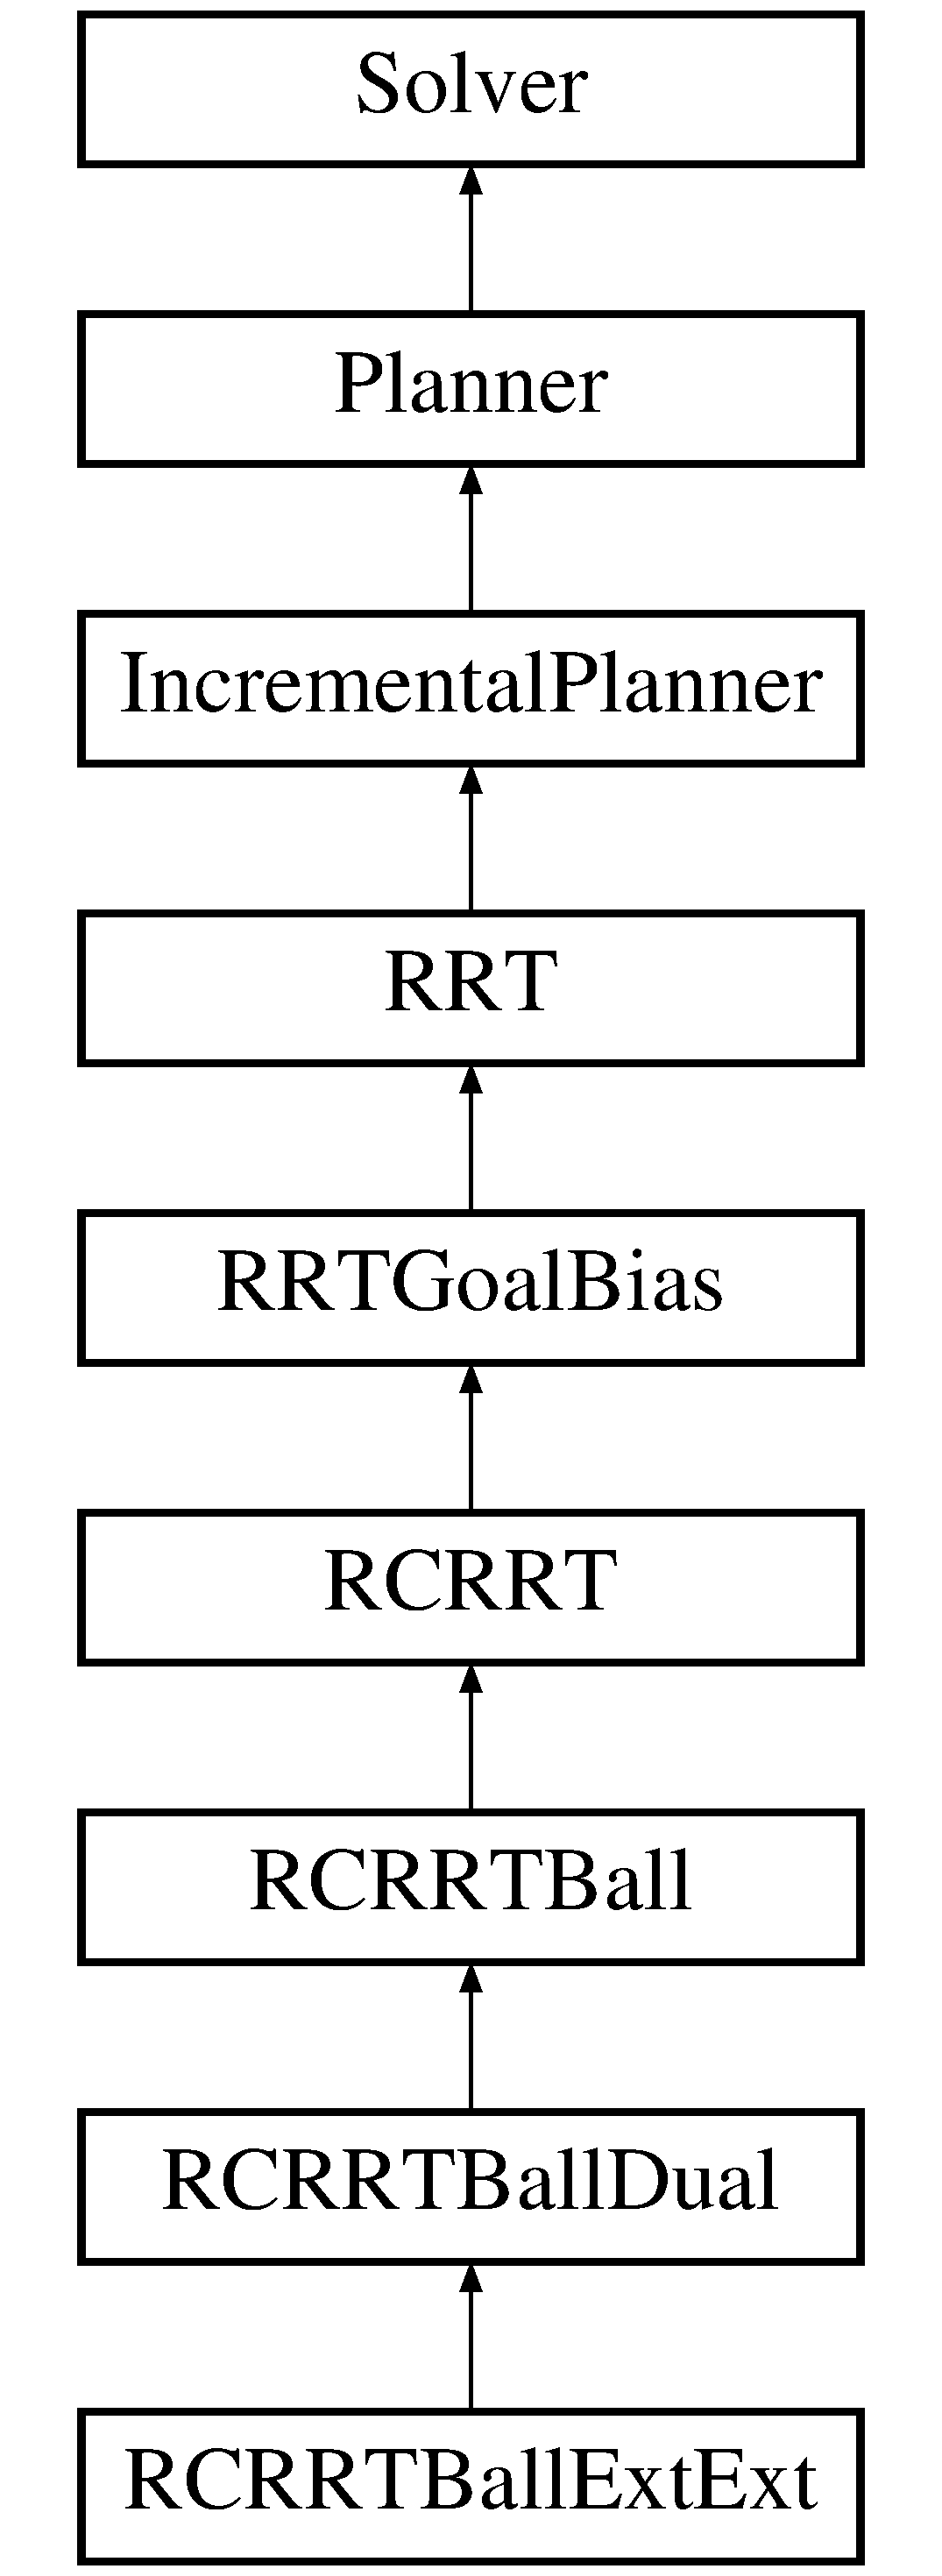
\includegraphics[height=9cm]{classRCRRTBall}
\end{center}
\end{figure}
\subsection*{Public Methods}
\begin{CompactItemize}
\item 
{\bf RCRRTBall} ({\bf Problem} $\ast$p)
\item 
virtual {\bf $\sim$RCRRTBall} ()
\item 
virtual {\bf MSLNode}$\ast$ {\bf Select\-Node} (const {\bf MSLVector} \&x, {\bf MSLTree} $\ast$t, bool forward)
\begin{CompactList}\small\item\em check the termination condition: n points in the balls in row.\item\end{CompactList}\item 
virtual bool {\bf Extend} (const {\bf MSLVector} \&x, {\bf MSLTree} $\ast$t, {\bf MSLNode} $\ast$\&nn, bool forward)
\begin{CompactList}\small\item\em Extend the nearest node to the random state.\item\end{CompactList}\item 
virtual bool {\bf Connect} (const {\bf MSLVector} \&x, {\bf MSLTree} $\ast$t, {\bf MSLNode} $\ast$\&nn, bool forward)
\begin{CompactList}\small\item\em extend the best input to a new state and check if the new state is in some balls.\item\end{CompactList}\item 
virtual bool {\bf Plan} ()
\begin{CompactList}\small\item\em Attempt to solve an Initial-Goal query by growing an {\bf RRT} {\rm (p.\,\pageref{classRRT})}.\item\end{CompactList}\end{CompactItemize}
\subsection*{Public Attributes}
\begin{CompactItemize}
\item 
double {\bf Ball\-Radius}
\begin{CompactList}\small\item\em the radius of the balls surrounding the nodes.\item\end{CompactList}\item 
int {\bf Fail\-Num\-Th}
\begin{CompactList}\small\item\em the termination number, if Fail\-Num random points are in the balls in row the algorithm terminates.\item\end{CompactList}\item 
int {\bf Fail\-Num}
\begin{CompactList}\small\item\em the number of times of the random points in the balls in row.\item\end{CompactList}\end{CompactItemize}


\subsection{Detailed Description}
{\bf RCRRT} {\rm (p.\,\pageref{classRCRRT})} planner using ball neighborhood to exclude the repeated states.



\subsection{Constructor \& Destructor Documentation}
\index{RCRRTBall@{RCRRTBall}!RCRRTBall@{RCRRTBall}}
\index{RCRRTBall@{RCRRTBall}!RCRRTBall@{RCRRTBall}}
\subsubsection{\setlength{\rightskip}{0pt plus 5cm}RCRRTBall::RCRRTBall ({\bf Problem} $\ast$ {\em p})}\label{classRCRRTBall_a0}


\index{RCRRTBall@{RCRRTBall}!~RCRRTBall@{$\sim$RCRRTBall}}
\index{~RCRRTBall@{$\sim$RCRRTBall}!RCRRTBall@{RCRRTBall}}
\subsubsection{\setlength{\rightskip}{0pt plus 5cm}RCRRTBall::$\sim$RCRRTBall ()\hspace{0.3cm}{\tt  [inline, virtual]}}\label{classRCRRTBall_a1}




\subsection{Member Function Documentation}
\index{RCRRTBall@{RCRRTBall}!Connect@{Connect}}
\index{Connect@{Connect}!RCRRTBall@{RCRRTBall}}
\subsubsection{\setlength{\rightskip}{0pt plus 5cm}bool RCRRTBall::Connect (const {\bf MSLVector} \& {\em x}, {\bf MSLTree} $\ast$ {\em t}, {\bf MSLNode} $\ast$\& {\em nn}, bool {\em forward} = true)\hspace{0.3cm}{\tt  [virtual]}}\label{classRCRRTBall_a4}


extend the best input to a new state and check if the new state is in some balls.



Reimplemented from {\bf RCRRT} {\rm (p.\,\pageref{classRCRRT_a9})}.\index{RCRRTBall@{RCRRTBall}!Extend@{Extend}}
\index{Extend@{Extend}!RCRRTBall@{RCRRTBall}}
\subsubsection{\setlength{\rightskip}{0pt plus 5cm}bool RCRRTBall::Extend (const {\bf MSLVector} \& {\em x}, {\bf MSLTree} $\ast$ {\em t}, {\bf MSLNode} $\ast$\& {\em nn}, bool {\em forward} = true)\hspace{0.3cm}{\tt  [virtual]}}\label{classRCRRTBall_a3}


Extend the nearest node to the random state.



Reimplemented from {\bf RCRRT} {\rm (p.\,\pageref{classRCRRT_a7})}.\index{RCRRTBall@{RCRRTBall}!Plan@{Plan}}
\index{Plan@{Plan}!RCRRTBall@{RCRRTBall}}
\subsubsection{\setlength{\rightskip}{0pt plus 5cm}bool RCRRTBall::Plan ()\hspace{0.3cm}{\tt  [virtual]}}\label{classRCRRTBall_a5}


Attempt to solve an Initial-Goal query by growing an {\bf RRT} {\rm (p.\,\pageref{classRRT})}.



Reimplemented from {\bf RCRRT} {\rm (p.\,\pageref{classRCRRT_a10})}.

Reimplemented in {\bf RCRRTBall\-Dual} {\rm (p.\,\pageref{classRCRRTBallDual_a2})}, and {\bf RCRRTBall\-Ext\-Ext} {\rm (p.\,\pageref{classRCRRTBallExtExt_a2})}.\index{RCRRTBall@{RCRRTBall}!SelectNode@{SelectNode}}
\index{SelectNode@{SelectNode}!RCRRTBall@{RCRRTBall}}
\subsubsection{\setlength{\rightskip}{0pt plus 5cm}{\bf MSLNode} $\ast$ RCRRTBall::Select\-Node (const {\bf MSLVector} \& {\em x}, {\bf MSLTree} $\ast$ {\em t}, bool {\em forward} = true)\hspace{0.3cm}{\tt  [virtual]}}\label{classRCRRTBall_a2}


check the termination condition: n points in the balls in row.



Reimplemented from {\bf RCRRT} {\rm (p.\,\pageref{classRCRRT_a6})}.

\subsection{Member Data Documentation}
\index{RCRRTBall@{RCRRTBall}!BallRadius@{BallRadius}}
\index{BallRadius@{BallRadius}!RCRRTBall@{RCRRTBall}}
\subsubsection{\setlength{\rightskip}{0pt plus 5cm}double RCRRTBall::Ball\-Radius}\label{classRCRRTBall_m0}


the radius of the balls surrounding the nodes.

\index{RCRRTBall@{RCRRTBall}!FailNum@{FailNum}}
\index{FailNum@{FailNum}!RCRRTBall@{RCRRTBall}}
\subsubsection{\setlength{\rightskip}{0pt plus 5cm}int RCRRTBall::Fail\-Num}\label{classRCRRTBall_m2}


the number of times of the random points in the balls in row.

\index{RCRRTBall@{RCRRTBall}!FailNumTh@{FailNumTh}}
\index{FailNumTh@{FailNumTh}!RCRRTBall@{RCRRTBall}}
\subsubsection{\setlength{\rightskip}{0pt plus 5cm}int RCRRTBall::Fail\-Num\-Th}\label{classRCRRTBall_m1}


the termination number, if Fail\-Num random points are in the balls in row the algorithm terminates.



The documentation for this class was generated from the following files:\begin{CompactItemize}
\item 
{\bf rcrrt.h}\item 
{\bf rcrrt.C}\end{CompactItemize}
